\pdfoptionpdfminorversion=7
\documentclass[11pt]{beamer}

\mode<presentation>
{
  \usetheme{Rochester}       % or try default, Darmstadt, Warsaw, ...
  \usecolortheme{default} % or try albatross, beaver, crane, ...
  \usefonttheme{serif}    % or try default, structurebold, ...
  \setbeamertemplate{navigation symbols}{}
  \setbeamertemplate{caption}[numbered]
}

\usepackage[utf8x]{inputenc}
\usepackage{booktabs} 
\usepackage{bibentry}
\usepackage{amsmath}
\usepackage{listings}
\usepackage{graphicx}
\usepackage{lmodern}
\usepackage{tikz}

\lstdefinestyle{mystyle}{
    breaklines=true,                 
    captionpos=b,                    
    keepspaces=true,                 
    numbers=left,                    
    numbersep=5pt,                  
    showspaces=false,                
    showstringspaces=false,
    showtabs=false,                  
    tabsize=2
}

\lstdefinestyle{MyStyleForCode}{
  language=Python,
  captionpos = b,
  showstringspaces=false,
  basicstyle=\tiny,
  keywordstyle=\bfseries\color{blue},
  commentstyle=\slshape\color{white!15!black},
  tabsize = 2,  
  stringstyle=\slshape\color{green!15!black},
  morekeywords = {class,self,open,from,import,map,list,sum,str,float,
  raw_input,abs,True,False,len,min,round,range,int,def,set},
  breaklines = True,
}

\title{Nueva propuesta para detección de contacto entre poliedros a gran escala}
\institute[Universidad Andrés Bello]{
\includegraphics[width=0.3\linewidth]{img/unab.png}
\hspace*{-0.5cm}~
}
\author{Yerko Zec}
\date{\today}


\begin{document}
\begin{frame}[plain]
  \titlepage
\end{frame}

\addtocounter{framenumber}{-1}

\begin{frame}{Contenido}
 \tableofcontents
\end{frame}


\section{Motivación}
\begin{frame}{Motivación}

     %\item Detección de contacto entre poliedros.
    % \item Simulación de grandes movimientos de rocas propuesto por Cundall \cite{1988-Cundall}.
     %\item Nueva propuesta para detección de contacto entre poliedros.
     %\item Problema de detección aún no se encuentra resuelto en su totalidad.
     
\end{frame}

\begin{frame}{prgunta de investigación}
    \begin{figure}[H]
        \begin{center}
            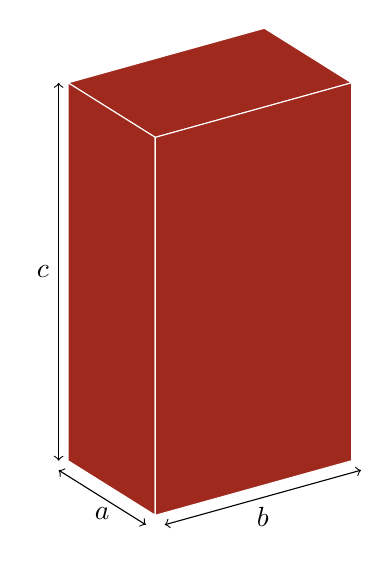
\begin{tikzpicture}[scale = 1.2]

                \pgfmathsetmacro{\cubex}{3}
                \pgfmathsetmacro{\cubey}{4}
                \pgfmathsetmacro{\cubez}{3}
                \pgfmathsetmacro{\x}{0}
                \pgfmathsetmacro{\y}{0}
                \pgfmathsetmacro{\z}{0}

                \definecolor{brick}{rgb}{0.62,0.16,0.11}

                \draw[white,fill=brick] (\x,\y,\z) -- ++(-\cubex/2,0,-\cubez/2) -- ++(\cubex/2,0,-\cubez/2) -- ++(\cubex/2,0,\cubez/2) -- cycle;
                \draw[white,fill=brick] (\x,\y,\z) -- ++(-\cubex/2,0,-\cubez/2) -- ++(0,-\cubey,0) -- ++(\cubex/2,0,\cubez/2) -- cycle;
                \draw[white,fill=brick] (\x,\y,\z) -- ++(0,-\cubey,0) -- ++(\cubex/2,0,-\cubez/2) -- ++(0,\cubey,0) -- cycle;

                \draw[<->,xshift = .1cm,yshift = -.1cm] (\x,\y -  \cubey,\z) -- ++(\cubex/2,0,-\cubez/2) node[midway,below] {$\mathlarger{b}$};
                \draw[<->,xshift = -.1cm,yshift = -.1cm] (\x,\y - \cubey,\z) -- ++(-\cubex/2,0,-\cubez/2) node[midway,below] {$\mathlarger{a}$};
                \draw[<->,xshift = -.1cm] (\x - \cubex/2,\y,\z - \cubez/2) -- ++(0.,-\cubey,0.) node[midway,left] {$\mathlarger{c}$};

            \end{tikzpicture}
        \caption{A rock represented by a regular polyhedron with dimensions $a$, $b$ and $c$.}
        \label{fig:rock}
        \end{center}
    \end{figure}
\end{frame}


\section{Marco teorico}
\begin{frame}{Marco teorico}
 \begin{itemize}
  \item En 1971 Cundall \cite{1988-Cundall} elaboró un método llamado Discrete Element Method(DEM).
  \item DEM está dividido en 3 fases: neighbor search, contact detection y force resolution.  
  \item Esta propuesta simula grandes movimiento de partículas.
  \item Hasta la fecha existen más de 15 algoritmos para la detección de contacto entre partículas.
  \begin{figure}[\centering]
    \includegraphics[width = 0.6\linewidth]{img/DEM}
  \end{figure}

 \end{itemize}
\end{frame}

\begin{frame}{Algunos algoritmos}
 \begin{itemize}
  \item En 1988 Cundall\cite{1988-Cundall} propuso un algoritmo llamado Common-Plane (CP)
  \item Mencionando algunos algoritmos utilizados a lo largo de la historia son: CP, FCP, MR, SLM, Multi-grid y MSC entre otros.
  \item Estos algoritmos empezaron desde la misma base que ocupa el algoritmo Common-Plane.
 \end{itemize}
\end{frame}

\begin{frame}{Common-Plane}
 \begin{itemize}
  \item Common-Plane(CP), fue en primera instancia creado por Cundall en 1988.
  \item Principio del algoritmo: Localizar un plano entre dos figuras e ir calculando la distancias.
  \begin{figure}[\centering]
  \includegraphics[width=0.5\linewidth]{img/CP}
  \end{figure}

 \end{itemize}
\end{frame}

\begin{frame}{Fast Common-Plane}
 \begin{itemize}
  \item En 2004 Nezami \cite{2004-Nezami} propuso una nueva propuesta para el cálculo del CP y se llamó Fast Common-Plane (FCP).
  \item Con esta nueva propuesta mejoró el orden del algoritmo por ello la eficiencia.
  \begin{figure}[\centering]
  \includegraphics[width = 0.5\linewidth]{img/Diagrama-FCP}
  \end{figure}

 \end{itemize}
\end{frame}

\begin{frame}{Shortest Link Method}
 \begin{itemize}
  \item Nezami en 2006 \cite{2006-Nezami} propuso otro algoritmo ocupando como base FCP.
  \item En base a resultados expuestos por Nezami \cite{2006-Nezami}, el SLM es 17 veces más rápido que otros algoritmos convencionales.
  \begin{figure}[\centering]
  \includegraphics[width=0.5\linewidth]{img/SLM}
  \end{figure}
 \end{itemize}
\end{frame}

\begin{frame}{Multi-shell Contact Detection}
 \begin{itemize}
  \item Fue desarrollado por Zhuang el 2014 \cite{2014-Zhuang}.
  \item La detección de contacto y la búsqueda de vecindario.
  \item MSC como método tanto de detección de vecindario como detección de contacto es uno de los más eficiente, según concluye Zhuang.
  \begin{figure}[\centering]
   \includegraphics[width=0.8\linewidth]{img/Multi-shell}
  \end{figure}
 \end{itemize}
\end{frame}

\section{Problema}
\begin{frame}{Problema}
    \begin{itemize}
        \item Detección de contacto computacionalmente costoso.
        \item Análisis de distintos tipos de colisiones.
    \end{itemize}
\end{frame}

\section{Objetivo}
\begin{frame}{Objetivo}

\begin{block}{Objetivo General}
 \begin{itemize}
    %\item Detectar de forma eficiente y eficaz el contacto entre poliedros.
    \item Desarrollar una nueva propuesta que detecte colisiones entre poliedros.
 \end{itemize}
\end{block}

\begin{block}{Objetivo Específico}
 \begin{itemize}
    \item Desarrollar una representación geométrica para los cuerpos rígidos.
    \item Desarrollar un algoritmo de detección de contactos para vértices y aristas.
    \item Desarrollar un algoritmo de detección de contacto entre cuerpos rígidos de orden no mayor a $\mathcal{O}(N)$, donde $N$ es la cantidad de cuerpos de la simulación.
 \end{itemize}
\end{block}
\end{frame}     

\section{Metodología}
\begin{frame}{Metodología}
\begin{itemize}
    \item Se realizó un estudio sobre el tema propuesto, donde se recopilaron los datos pertinentes.
    \item Se generó una línea de tiempo donde se señalaron los trabajos más relevantes al tema.
    \item Desarrollo de algoritmo en 2-D.
    \item Upgrade del algoritmo a 3-D.
    \item Optimización de codigo, con el fin de probar un set de prueba
    \color{red} Cambiar el ultimo punto para que se entienda mejor.
\end{itemize}
\end{frame}

\begin{frame}{Metodología}
\begin{itemize}
    \item Principales framework de trabajo son github, pycharm, kile y overleaf.
\end{itemize}
    \begin{figure}
     \includegraphics[width = 0.2\linewidth]{img/github_logo}
     \includegraphics[width = 0.2\linewidth]{img/pycharm}
     \includegraphics[width = 0.2\linewidth]{img/kile}
     \includegraphics[width = 0.2\linewidth]{img/Overleaf}
    \end{figure}
\end{frame}

\begin{frame}{Metodología}
\begin{itemize}
    \item Para el control de versiones del código se utilizó un repositorio en github.
    \begin{figure}
      \includegraphics[width = 1\linewidth]{img/github}
    \end{figure}

\end{itemize}
\end{frame}

\section{Resultados}
\begin{frame}{Resultados}
 \begin{block}{Código 2-D}
  \lstinputlisting[style = MyStyleForCode, 
  frame = single,
  firstline = 7, 
  lastline = 23, 
  label= {lst:Get_var}]{Codigo/3d_figure_detection.py}
 \end{block}
\end{frame}

\begin{frame}{Resultados}
 \begin{block}{Detección de punto}
  \lstinputlisting[style = MyStyleForCode, 
  frame = single,
  firstline = 69, 
  lastline = 92, 
  label= {lst:Get_var}]{Codigo/3d_figure_detection.py}
 \end{block}
\end{frame}

\begin{frame}{Resultados}
 \begin{block}{Prueba 2-D}
\begin{figure}
 \includegraphics[width = 0.6\linewidth]{img/Figura_arista}
 \includegraphics[width = 0.6\linewidth]{img/Figura_dentro}
\end{figure}
 \end{block}
\end{frame}

\begin{frame}{Resultados}
 \begin{block}{Prueba 2-D}
\begin{figure}
 \includegraphics[width = 0.6\linewidth]{img/Figura_vertice}
 \includegraphics[width = 0.6\linewidth]{img/figura_fuera}
\end{figure}
 \end{block}
\end{frame}

\begin{frame}{Resultados}
 \begin{block}{Codigo 3-D}
  \lstinputlisting[style = MyStyleForCode, 
  frame = single,
  firstline = 6, 
  lastline = 28, 
  label= {lst:Get_var}]{Codigo/detection-3d.py}
 \end{block}
\end{frame}

\begin{frame}{Resultados}
 \begin{block}{Codigo 3-D}
  \lstinputlisting[style = MyStyleForCode, 
  frame = single,
  firstline = 66, 
  lastline = 92, 
  label= {lst:Get_var}]{Codigo/detection-3d.py}
 \end{block}
\end{frame}

\begin{frame}{Resultados}
 \begin{block}{Prueba 3-D}
    \begin{figure}
        \includegraphics[width = 0.45\linewidth]{img/3Dprueba1}
        \includegraphics[width = 0.45\linewidth]{img/3Dprueba2}
    \end{figure}
 \end{block}
\end{frame}

\begin{frame}{Resultados}
 \begin{block}{Prueba 3-D}
    \begin{figure}
        \includegraphics[width = 0.45\linewidth]{img/3Dprueba3}
        \includegraphics[width = 0.45\linewidth]{img/3Dprueba5}
    \end{figure}
 \end{block}
\end{frame}

\section{Conclusi\'on}
\begin{frame}{Conclusión}
 \begin{itemize}
  \item 
  \item En esta fase del desarrollo de la propuesta se logr\'o detectar si un vértice y una arista están en contacto con el poliedro.
 \end{itemize}
\end{frame}

\section{Referencias}
\begin{frame}{Referencias}
\medskip
\bibliographystyle{plain}
\bibliography{/files/Referencia}
\end{frame}


\begin{frame}[plain]
  \titlepage
\end{frame}

\end{document}
